\chapter{Spin transport in long-range anisotropic Heisenberg model\label{chap:spin_transport}}
\thispagestyle{chapterBeginStyle}

After all the technicalities of the previous chapter, we are finally ready to study spin transport in
the long-range anisotropic Heisenberg model. The main motivation of this investigation is the fact that this model admits 
two limits exhibiting ballistic spin transport (cf. Fig.~\ref{fig:spin_transport}), namely the free particles
with nearest-neighbor hopping for \(\alpha\to \infty,\; \Delta = 0\) and (in the thermodynamic limit) the Haldane-Shastry
model for \(\alpha = 2\)~\autocite{Haldane1988,Shastry1988}. In both of these limiting models the spin current 
\(j^{\sigma}\) commutes with the Hamiltonian and thus is strictly conserved. Thus, even though
the Hamiltonian~\eqref{eq:long_range} is not integrable for arbitrary \(\alpha\), one could suspect
that it will be \textit{nearly integrable}, in the sense described in the introduction, and support
interesting transport properties. Using spin density expansion and linear response theory of optical conductivity,
in this chapter we will show that this is indeed the case and the spin transport is \textit{quasibalistic} along a sharp
line in the parameter space \(\Delta \simeq \exp(- \alpha + 2)\), which continuously connects the two limiting
cases mentioned above.

Results described in this chapter were first presented in chapters II and III of ~\textcite{Mierzejewski2023}.

\begin{figure}[htbp]
    \centering
    \begin{tikzpicture}[scale=1.5]
      \colorlet{col1}{blue!30}
    
     \begin{scope}[smooth,draw=gray!20,y=0.3989422804cm]
          \filldraw[fill=col1] plot[id=f1, domain=-1.5:1.5,samples=100] function {6*exp(-6*x*x)};
          \draw[black] plot[id=f2,domain=-1.5:1.5,samples=100]
              function {6*exp(-6*x*x)};
      \end{scope}
      \draw[->] (-1.5,0) -- (1.5,0) node [right] {$x$};
      \draw[->] (-1.5,0) -- (-1.5,2.5) node [midway,rotate=90,yshift=6pt] {spin density};
      \draw[<->] (-0.37,1) -- (0.37,1) node [midway, yshift=6pt] {$\gamma$};
    
      \begin{scope}[smooth,draw=gray!20,y=0.3989422804cm]  
        \draw[black] plot[id=f3,domain=2.35:5.35,samples=100] function {0.7};    
        \draw[black] plot[id=f4,domain=2.35:5.35,samples=100] function {x};    
        \draw[black] plot[id=f5,domain=2.35:5.35,samples=100] function {sqrt(x)};    
      \end{scope}  
      
      \draw[->] (2.35,0) -- (5.35,0) node [right] {$t$};
      \draw[->] (2.35,0) -- (2.35,2.5) node [right] {$\gamma$};
      \node[draw=none] at (3.35,1.6) {$\gamma \propto t$};
      \node[draw=none] at (3.45,0.95) {$\gamma \propto \sqrt{t}$};
      \node[draw=none] at (3.6,0.4) {$\gamma = const$};
      \node[draw=none] (localized) at (6,0.3) {localized};
      \node[draw=none,above of=localized,node distance=27pt] (diffusive) {diffusive};
      \node[draw=none,above of=diffusive,node distance=45pt] (ballistic) {ballistic};
    \end{tikzpicture}  
    \caption{Illustration of different types of transport. On the left panel, we have some initial spin
    density characterized by width \(\gamma\). On the right panel, we have the dependence of \(\gamma\)
    on time in three different cases.}
    \label{fig:spin_transport}
  \end{figure}
  
  \section{Spin density expansion}

  Taking inspiration from experimental studies of cold atoms~\autocite{Joshi2022, Ronzheimer2013, Vidmar2013, Neyenhuis2017},
  we consider an initial state in the form of a spin domain wall
  \begin{equation}
    \ket{\psi(0)} = \ket*{\underbrace{\uparrow\uparrow\uparrow\uparrow\uparrow}_{x}
    \underbrace{\downarrow\downarrow\downarrow\ldots\downarrow}_{L-x}},\; x = 5
  \end{equation}
and study the dynamics of spin expansion by measuring the time dependence of the magnetization profile
\(M_{\ell}(t) = \matrixel{\psi(t)}{\Sz_{\ell}}{\psi(t)}\). Such a product state initial configuration is desirable for two reasons.
First, it is relatively accessible in experiments, e.g. using higher-order optical Stark shifts to rotate individual
spins~\autocite{Lee2016}. Second, from the theoretical point of view, by assuming open boundary conditions and
choosing \(x = 5\), we localize the domain wall close to the edge of the system, which allows us to avoid finite-size effects
for longer times. Moreover, the dynamics generated by the Hamiltonian~\eqref{eq:long_range} conserve the total magnetization
and hence we can restrict ourselves to the subspace of states with just five up spins. This considerably reduces
the dimensionality of the problem and allows us to study a system as large as \(L=45\) with
\(\binom{45}{5} \approx 1.2 \times 10^6\) states, characterized by the total magnetization \(M_{\mathrm{tot}} = -35/2\).
To put this into perspective, the full Hilbert space of the system
has dimension \(2^{45}\) which is \(O(10^7)\) larger and thus completely inaccessible without additional techniques.

For the time evolution, we use the Krylov propagator introduced in detail in the previous chapter.
A sample magnetization profile obtained for \(\alpha = 3.5\) and \(\Delta = 1.0\) is shown in 
Fig.~\ref{fig:magnetization_profile}.
\begin{figure}[htbp]
  \centering
  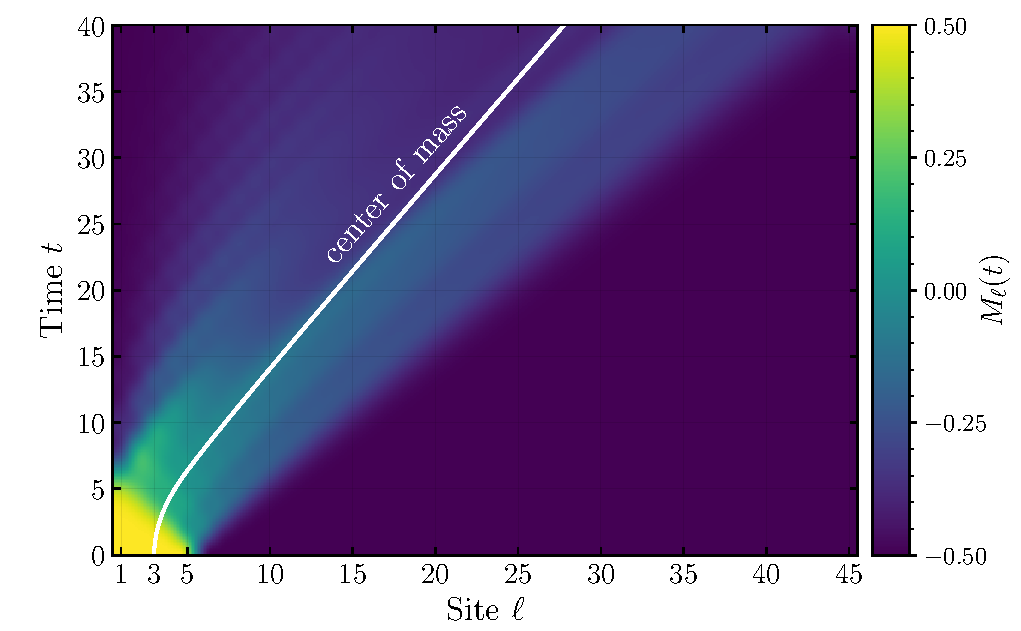
\includegraphics[width=0.9\linewidth]{Figures/magnetization.pdf}
  \caption{Time dependence of magnetization profile \(M_{\ell}(t)\) for \(\alpha = 3.5\) and \(\Delta = 1.0\).
  The evolution of the center of mass, initially at \(r_{\text{cm}}(t=0)=3\), is marked by a white line.}
  \label{fig:magnetization_profile}
\end{figure}
\newpage
In order to quantitatively investigate the spin transport in this setup, we introduce the so-called
\textbf{center of mass}, defined as the first density moment of the magnetization profile  
\begin{equation}
  r_{\text{cm}}(t) = \frac{\sum_{\ell=1}^{L} \ell \left(M_{\ell}(t)+1/2\right)}
  {\sum_{\ell=1}^{L} \left(M_{\ell}(t) + 1/2\right)} = 
\frac{\sum_{\ell=1}^{L} \ell \left(M_{\ell}(t)+1/2\right)}
  {M_{\mathrm{tot}} + L/2}
  \label{eq:center_of_mass} 
\end{equation}
A sample trajectory of the center of mass is shown in Fig.~\ref{fig:magnetization_profile}. Examining \(r_{\text{cm}}(t)\)
calculated for two values of \(\Delta = 0.2,\;0.5\) and various values of \(\alpha \in \{2.0,2.5,\ldots,5.0\}\)
(cf. Fig.~\ref{fig:center_of_mass}), we observe a first hint of non-trivial transport properties of the model, namely
non-monotonic dependence of \(r_{\text{cm}}(t)\) on \(\alpha\). 

\begin{figure}[htbp]
  \centering
  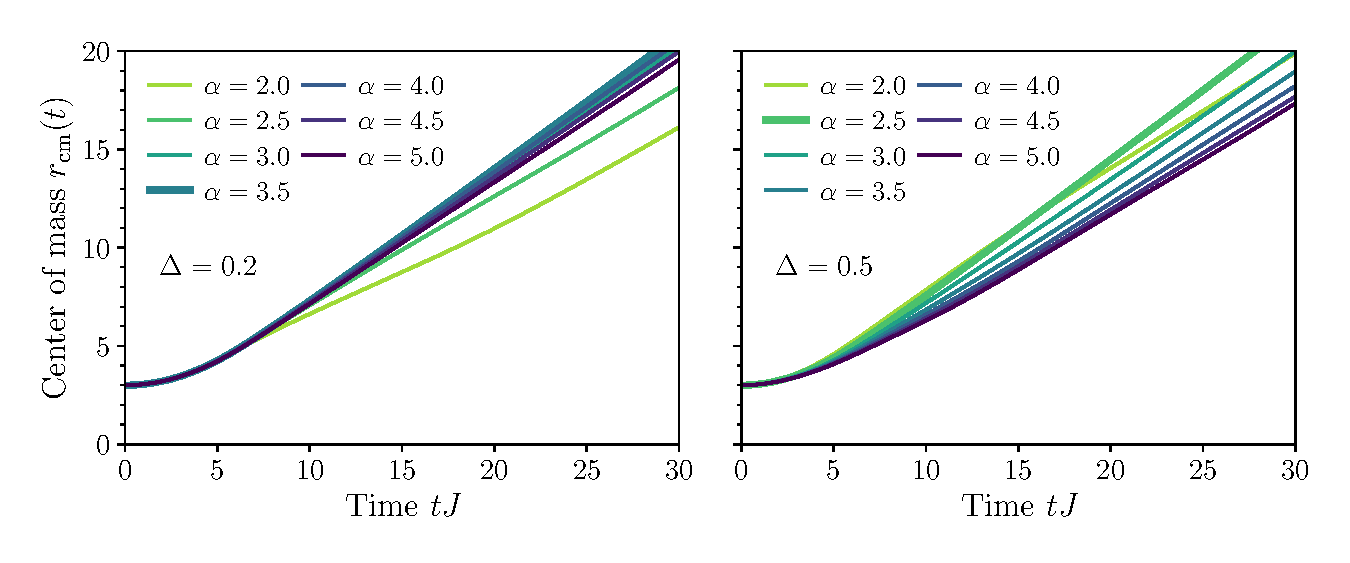
\includegraphics[width=\linewidth]{Figures/center_of_mass.pdf}
  \caption{Time dependence of the center of mass \(r_{\text{cm}}(t)\) for \(\Delta = 0.2\) (left panel) and \(\Delta = 0.5\)
  (right panel) and various values of interaction decay \(\alpha\). The line corresponding to the fastest moving center of mass
  is thicker than the others.}
  \label{fig:center_of_mass}
\end{figure}

To see this better, we also look at the velocity
obtained from the time derivative of the center of mass
\begin{equation}
  v_{\text{cm}}(t) = \dv{r_{\text{cm}}(t)}{t}.
  \label{eq:velocity}
\end{equation}



\textcolor{red}{optimal alpha for a given delta, giving largest velocity}
\textcolor{red}{average velocities and delta-alpha heatmap}



\section{Optical conductivity}






\textcolor{red}{Mention similarity to non interacting fermions.}
\textcolor{red}{Mention that this quasibalistic transport is characteristic for long range,
and is not present in NNN, or generalized HS and this is investigated in the paper.}